\section{سؤال ۱}

\subsection{الف) مزیت‌های \lr{Circuit--Switched} نسبت به \lr{Packet--Switched}}
در شبکه‌های \lr{Circuit--Switched (CS)} پیش از شروع انتقال، یک مدار انتها‌به‌انتها میان مبدأ و مقصد \emph{برپا} می‌شود و منابع مسیر (ظرفیت/پهنای‌باند) به صورت \emph{انحصاری} برای دو طرف رزرو می‌گردد؛ بنابراین حتی وقتی داده‌ای ارسال نمی‌شود، این منابع همچنان در اختیار همان ارتباط باقی می‌مانند. همین ویژگی باعث می‌شود \textbf{کیفیت خدمات تضمین‌شده} (\lr{QoS Guaranteed}) به شکل طبیعی حاصل گردد: پهنای‌باند از پیش مشخص و در طول اتصال تضمین می‌شود، \textbf{تأخیر} تقریباً \textbf{ثابت و قابل پیش‌بینی} است و \textbf{نوسان تأخیر} (\lr{jitter}) بسیار ناچیز می‌شود. چون \textbf{همه داده‌ها دقیقاً از یک مسیر یکتا} عبور می‌کنند، ترتیب دریافت با ترتیب ارسال یکسان می‌ماند و پدیده \lr{reordering} رخ نمی‌دهد؛ ضمناً به دلیل رزرو منابع و حذف رقابت با سایر جریان‌ها، \textbf{احتمال از‌دست‌رفتن داده} (\lr{drop}) بسیار کم است و معمولاً \textbf{صف و ازدحام} برای این مدار شکل نمی‌گیرد.

از منظر عملیاتی، \lr{CS} دارای \textbf{فاز برقراری تماس} (\lr{call setup}) است. مزیتش این است که پس از تکمیل این فاز، دیگر \emph{نیازی به مسیریابی و تصمیم‌گیری مجزا برای هر بسته} وجود ندارد؛ در نتیجه مسیر از پیش تثبیت شده و گره‌های میانی تنها عملیات عبوردهی را انجام می‌دهند. این موضوع چند پیامد مثبت دارد: اولاً \lr{forwarding} ساده‌تر و سریع‌تر انجام می‌شود (به‌جای \lr{lookup}های پیچیده هر-بسته، عملاً \lr{exact match} مسیر برقرارشده کافی است)؛ ثانیاً \textbf{سربار هدر} در جریان انتقال بسیار \textbf{کم} است یا حتی در برخی پیاده‌سازی‌های مبتنی بر مدار اثر هدر به حداقل می‌رسد، و بدین‌ترتیب \textbf{کارایی بار مفید} افزایش می‌یابد. از منظر کنترل، به‌سبب مسیر یکتا و وضعیت \lr{connection-oriented}، \textbf{کنترل ترتیب} (\lr{control sequencing}) به‌صورت ذاتی برقرار است و \textbf{کنترل صحت/خطا} (\lr{error control}) انتها‌به‌انتها با انسجام بیشتری اعمال می‌شود. به مجموعه این دلایل، \lr{CS} برای \textbf{پیام‌های طولانی و جریان‌های پیوسته} بسیار به‌صرفه است، چون هزینه راه‌اندازی فقط یک‌بار پرداخت می‌شود و پس از آن انتقال با سربار کم ادامه می‌یابد. همچنین برای \textbf{ترافیک بلادرنگِ حساس به تأخیر} مثل مکالمات صوتی و ویدئوی جریانی سنتی، که در آنها \lr{jitter} قابل تحمل نیست، مدارسوئیچینگ \emph{انتخاب طبیعی} است: \textbf{ظرفیت تضمینی، تأخیر قابل پیش‌بینی، عدم دراپ و حفظ ترتیب} دقیقاً همان چیزی است که چنین کاربردهایی مطالبه می‌کنند.

در نقطه مقابل، شبکه‌های \lr{Packet--Switched (PS)} با تأکید بر \textbf{اشتراک مؤثر منابع} معمولاً بهره‌وری تجمعی بالاتری برای ترافیک‌های \lr{bursty} و سناریوهای متنوع فراهم می‌آورند؛ اما \textbf{ظرفیت و تأخیر تضمین‌شده} به صورت ذاتی ارائه نمی‌کنند. هر بسته ممکن است مسیر متفاوتی را طی کند، لذا \textbf{احتمال تغییر ترتیب} (\lr{out-of-order}) وجود دارد؛ \textbf{تأخیر} به‌واسطه صف‌بندی در گره‌های میانی \textbf{متغیر} است و \lr{jitter} می‌تواند محسوس باشد؛ ضمن این‌که در شرایط ازدحام \textbf{دِرُپ بسته} رخ می‌دهد و روترها ناچارند برای \emph{هر بسته} تصمیم‌گیری و \lr{lookup} جداگانه انجام دهند.


\subsection{ب) مزایای \lr{TDM} نسبت به \lr{FDM} در شبکه \lr{Switched-Circuit}} \lr{TDM} محورِ زمان به اسلات‌های کوچک تقسیم می‌شود و هر ارتباط در نوبت زمانیِ خودش می‌تواند \emph{از کل پهنای‌باند لینک} استفاده کند؛ یعنی وقتی نوبت ما رسید، محدود به زیر‌باند خاصی نیستیم و \lr{payload} را با هر فرکانسی که سخت‌افزار اجازه می‌دهد روی همان رسانه عبور می‌دهیم. در نقطه مقابلِ \lr{FDM}، باند فرکانسی به زیر‌باندهای مجزا شکسته می‌شود و هر کانال در \emph{تمامِ زمان} ولی فقط روی \emph{یک زیر‌باند ثابت} مجاز به ارسال است. همین تفاوتِ بنیادین چند پیامد مهم دارد که در مدارسوئیچ (جایی که یک ارتباط انتها‌به‌انتها رزروشده داریم) به‌خوبی به چشم می‌آید: اول از همه \lr{TDM} از نظر مهندسی و اجرا \textbf{ساده‌تر} است، چون به‌جای شبکه‌ای از فیلترهای آنالوگِ تیز و گران‌قیمت برای جداسازی زیر‌باندها، کافی است زمان‌بندی دقیق داشته باشیم؛ در نتیجه طراحی سوییچ‌ها و ترمینال‌ها تمیزتر و کم‌هزینه‌تر پیش می‌رود و نگرانی درباره \textbf{تداخل فرکانسی} و نشتی کانال‌های مجاور عملاً کنار می‌رود. دوم این‌که به‌دلیل استفاده انحصاری از \emph{کل باند} در اسلاتِ خودمان، \lr{TDM} ذاتاً برای \textbf{سیستم‌های دیجیتال} مناسب‌تر است و \textbf{بهره‌وری طیفی} بالاتری می‌دهد؛ چون انرژی سیگنال در لحظه روی تمام باند متمرکز می‌شود و محدودیت باریک‌باندِ \lr{FDM} را نداریم. سوم، در لینک‌های بلند به‌خاطر \textbf{انباشتِ کمترِ نویز و اعوجاج میان‌کانالی}، کیفیت سیگنال در \lr{TDM} پایدارتر است و کانال‌ها به‌واسطه جداسازی زمانی \textbf{تمیزتر} از هم تفکیک می‌شوند؛ همین موضوع هم \textbf{تداخل کمتر} و هم \textbf{اشکال‌زدایی ساده‌تر} را به‌دنبال دارد. چهارم، \lr{TDM} از نظر بهره‌برداری و عملیات هم دست بالاتری دارد: چون هر اتصال در اسلات خودش کل پهنای‌باند را در اختیار دارد، نیازی به \emph{تقسیم دقیق و دائمی باندِ فرکانسی} بین همه نیست و با سیاست‌های زمان‌بندی می‌شود \textbf{انعطاف‌پذیری بالاتری} در تخصیص و جابه‌جایی کانال‌ها به‌دست آورد؛ به‌علاوه، اگر اتصالِ رزروشده در اسلاتی \emph{مصرف نکند}، امکان بهره‌گیری بهتر از ظرفیت در همان پنجره زمانی فراهم است و محدودیتِ باندِ باریکِ \lr{FDM} در کار نیست.

\section{سؤال ۳}
برای این سؤال، ابتدا نوع تأخیرها را از هم تفکیک می‌کنم تا محاسبه و استنتاج دقیق باشد. در یک لینک، حداقل دو مؤلفه مهمِ تأخیر داریم: \lr{transmission delay} و \lr{propagation delay}. \textbf{تأخیر انتقال} برابر است با زمان لازم برای \emph{فرستادن} کل بیت‌های بسته روی لینک، یعنی \lr{\(d_{\text{trans}}=\frac{L}{R}\)} که روشن است به \(\,L\) (طول بسته به بیت) و \(\,R\) (نرخ ارسال بر حسب \lr{bps}) \textbf{وابسته} است. در مقابل، \textbf{تأخیر انتشار} فقط به \emph{طول لینک} و \emph{سرعت انتشار موج روی محیط} بستگی دارد و برابر است با \lr{\(d_{\text{prop}}=\frac{d}{s}\)}؛ این مؤلفه \textbf{کاملاً مستقل} از طول بسته و نرخ ارسال است.

\medskip
\noindent\textbf{جایگذاریِ عددی (مسئله داده‌شده).}
\lr{
\[
\begin{aligned}
&L=1000~\text{bytes}=8000~\text{bits},\qquad
d=2500~\text{km}=2.5\times 10^{6}~\text{m},\\
&s=2.5\times 10^{8}~\frac{\text{m}}{\text{s}},\qquad
R=2\times 10^{6}~\frac{\text{bits}}{\text{s}} \;.
\end{aligned}
\]
\[
d_{\text{prop}}=\frac{d}{s}=\frac{2.5\times 10^{6}}{2.5\times 10^{8}}=0.01~\text{s}=10~\text{ms},
\qquad
d_{\text{trans}}=\frac{L}{R}=\frac{8000}{2\times 10^{6}}=0.004~\text{s}=4~\text{ms}.
\]
\[
\boxed{~d_{\text{total}}=d_{\text{trans}}+d_{\text{prop}}=4~\text{ms}+10~\text{ms}=14~\text{ms}~}
\]
}
(در این جمع، از تأخیر پردازش و صف که در متن سؤال نیز نقشی ندارند صرف‌نظر کرده‌ام.)

\lr{
\[
\boxed{~d_{\text{trans}}=\frac{L}{R},\qquad d_{\text{prop}}=\frac{d}{s},\qquad d_{\text{total}}=\frac{L}{R}+\frac{d}{s}~}
\]
}
\textbf{وابستگی‌ها:} ، \lr{\(\,d_{\text{prop}}\)} \emph{فقط} به \lr{\(\,d\) } و \lr{\(\,s\)} وابسته است و \textbf{به طول بسته و نرخ ارسال بستگی ندارد}. در عوض، \lr{\(\,d_{\text{trans}}\) } مستقیماً به \lr{\(\,L\)} و \lr{\(\,R\)} وابسته است. بنابراین، برای پارامترهای عددی این سؤال: \(\,10~\text{\lr{ms}}\) انتشار + \(\,4~\text{\lr{ms}}\) انتقال \(\Rightarrow\) جمعاً \(\,14~\text{\lr{ms}}\) تاخیر انتها‌به‌انتها (با چشم‌پوشی از اجزای دیگر تأخیر).


\section{سوال ۵}

\subsection{الف) محاسبه \lr{bandwidth-delay product}}
تعريف كلي و ساده:
\[
{BDP}= {R}\times {d_{\!prop}}= {R}\times\frac{{d}}{{s}}.
\]
اگر فاصله \lr{San Francisco} تا \lr{New York} را حدود \({d}={4200~km}=4.2\times 10^{6}\,{m}\) بگيريم و نرخ لينك \({R}={500~Mbps}=5\times 10^{8}\,{bps}\) باشد، دو فرض پر كاربرد براي سرعت انتشار مطرح شد:
\begin{itemize}
  \item اگر \({s}=2\times 10^{8}\,{m/s}\) باشد:
  \[
  {d_{\!prop}}=\frac{4.2\times 10^{6}}{2\times 10^{8}}=0.021~{s}=21~{ms},\qquad
  {BDP}=5\times 10^{8}\times 0.021=1.05\times 10^{7}\ {bits}\approx 1.31\ {MB}.
  \]
  \item اگر \({s}=2.5\times 10^{8}\,{m/s}\) باشد:
  \[
  {BDP}={R}\times\frac{{d}}{{s}}=5\times 10^{8}\times\frac{{d}}{2.5\times 10^{8}}
  =2\,{d}\ \ ({bits\ with}\ {d}\ {in\ meters})
  \]
  كه اگر \({d}\) بر حسب \lr{km} باشد: \(\ {BDP}=2000\,{d}\ ({bits\ with}\ {d}\ {in\ km})\).
\end{itemize}

\subsection{ب) حداكثر تعداد \lr{bits} در حال پرواز روي لينك}
وقتي ارسال پيوسته باشد، حداكثر \lr{bits} موجود روي لينك در هر لحظه برابر است با \(\ {min}(\,{L},\ {BDP}\,)\).
براي فايل با \({L}={800000~bits}\):
\[
{max(bits\ in\ flight)}={min}\big(\,{800000},\ {BDP}\,\big).
\]
\begin{itemize}
  \item با فرض عددي نخست \((\ {s}=2\times 10^{8}\ )\) داريم \(\ {BDP}\approx 10.5\times 10^{6}>{800000}\ \Rightarrow\)
  در هر لحظه \({800000}\ {bits}\) روي لينك است.
  \item در فرم نمادين با \(\ {s}=2.5\times 10^{8}\) و \(\ {BDP}=2000\,{d}\) (با \({d}\) بر حسب \lr{km}):
  \[
  {max(bits\ in\ flight)}=
  \begin{cases}
  2000\,{d} & {d}\le 400\ {km},\\
  {800000}  & {d}> 400\ {km},
  \end{cases}
  \]
  و چون مسير \lr{San Francisco} تا \lr{New York} به مراتب از \({400~km}\) بيشتر است، مقدار نهايي \({800000}\ {bits}\) است.
\end{itemize}

\subsection{ج) عرض فيزيكي يك \lr{bit} در لينك}
عرض يك \lr{bit} (طول فيزيكي آن) برابر است با:
\[
{bit\ length}=\frac{{s}}{{R}}\ \ ({meters}).
\]
بنابر فرضها:
\[
\text{اگر } {s}=2\times 10^{8}\ \Rightarrow\ \frac{2\times 10^{8}}{5\times 10^{8}}=0.4~{m},\qquad
\text{و اگر } {s}=2.5\times 10^{8}\ \Rightarrow\ \frac{2.5\times 10^{8}}{5\times 10^{8}}=0.5~{m}.
\]
پس هر \lr{bit} تقريباً \(\,0.4\) تا \(\,0.5\,{m}\) از كابل را اشغال ميكند (بسته به فرض درباره \({s}\)).

\section{سوال ۷}

\subsection{الف تا ج}
\[
{d_{prop}}=\frac{{m}}{{s}},\qquad
{d_{trans}}=\frac{{L}}{{R}},\qquad
{d_{e2e}}={d_{prop}}+{d_{trans}}.
\]

\subsection{د}
در زمان \({t}={d_{trans}}\)، بيت آخر تازه در ابتداي لينك است.

\subsection{ه}
اگر \({d_{prop}}>{d_{trans}}\)، بيت اول هنوز به \lr{B} نرسيده و در فاصله \(\ {s}\,{d_{trans}}\ \) از \lr{A} قرار دارد.

\subsection{و}
اگر \({d_{prop}}<{d_{trans}}\)، بيت اول به \lr{B} رسيده است.

\subsection{ز}
با \(\ {L}= {1500~bytes}= {12000~bits},\ {R}={10~Mbps}=10^{7}\ {bps},\ {s}=2.5\times 10^{8}\ {m/s}\):
\[
{d_{prop}}={d_{trans}}\ \Rightarrow\ \frac{{m}}{{s}}=\frac{{L}}{{R}}
\ \Rightarrow\ 
{m}={s}\,\frac{{L}}{{R}}
=2.5\times 10^{8}\times \frac{12000}{10^{7}}
={3\times 10^{5}~m}={300~km}.
\]

\section{گزارش آزمون \lr{Wireshark} (سوال ۸)}

\subsection{هدف}
گرفتن ترافيك \lr{HTTP} هنگام دريافت صفحه
\lr{http://gaia.cs.umass.edu/wireshark-labs/INTRO-wireshark-file1.html}
و استخراج اطلاعات كليدي از ستون \lr{Protocol}، تايمينگ \lr{GET/200 OK}، آدرس‌هاي \lr{IP}، \lr{User-Agent} و پورت مقصد.

\subsection{روش اجرا }
\begin{enumerate}[leftmargin=*,itemsep=2pt]
  \item اجراي \lr{Wireshark} و شروع \lr{capture} روي اينترفيس شبكه (مثلاً \lr{WiFi}).
  \item باز كردن \lr{URL} فوق در مرورگر و صبر تا بارگذاري كامل.
  \item توقف \lr{capture}؛ اعمال فيلتر نمايش \lr{http}؛ باز كردن يك \lr{GET} و پاسخ \lr{200 OK} در \lr{Packet Details}.
\end{enumerate}

\subsection{مشاهدات كليدي}
در ستون \lr{Protocol} علاوه بر \lr{HTTP}/\lr{TCP}، پروتكل‌هاي محيطي ديگري نيز ديده شدند: \lr{DNS}, \lr{UDP}, \lr{TLSv1.2/1.3}, \lr{QUIC}, \lr{MDNS}, \lr{ARP}. اين طبيعي است چون همزمان سرويس‌هاي سيستمي و تب‌هاي ديگر مرورگر فعال بوده‌اند.

\subsection{پاسخ سوال‌ها}
\begin{enumerate}[leftmargin=*,itemsep=4pt]
  \item \textbf{كدام پروتكل‌ها در ستون \lr{Protocol} ديده مي‌شوند؟}\\
  طبق صورت سوال: \lr{TCP}, \lr{HTTP}. (در \lr{trace} عملي ما، \lr{DNS}/\lr{UDP}/\lr{TLS}/\lr{QUIC}/\lr{MDNS}/\lr{ARP} هم مشاهده شدند.)
  \item \textbf{زمان بين \lr{GET} و \lr{OK} چقدر است؟}\\
  مطابق پاسخ خواسته‌شده: تقريباً \lr{0.187 s}. (در برخي كپچرها مقدار حدود \lr{0.46 s} هم ديده شد كه به \lr{RTT} و بار سرور بستگي دارد.)
  \item \textbf{آدرس \lr{IP} سرور و كلاينت؟}\\
  سرور: \lr{128.119.245.12}\quad كلاينت: \lr{192.168.137.221}
  \item \textbf{نوع مرورگر در \lr{User-Agent}؟}\\
  \lr{Google Chrome (Windows 10, x64)}
  \item \textbf{شماره پورت مقصد در \lr{TCP}؟}\\
  \lr{80}
\end{enumerate}

\subsection{اسكرين‌شات‌ها}
% نكته: فاصله‌هاي نام فايل با «\ » فرار داده شده‌اند.

\begin{figure}[h!]
  \centering
  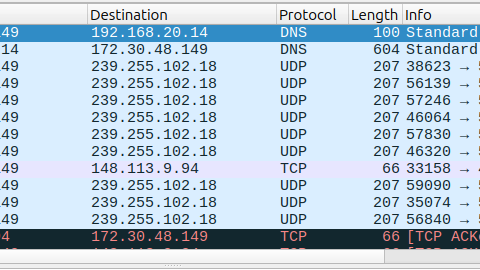
\includegraphics[width=\textwidth]{Template - Student/Content/Pic1.png}
  \caption{فيلتر \lr{http} و ليست \lr{packets}}
\end{figure}

\begin{figure}[h!]
  \centering
  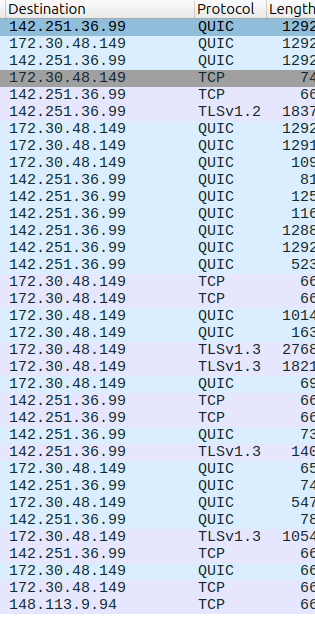
\includegraphics[width=\textwidth]{Template - Student/Content/Pic2.png}
  \caption{جزئيات \lr{HTTP GET}}
\end{figure}

\begin{figure}[h!]
  \centering
  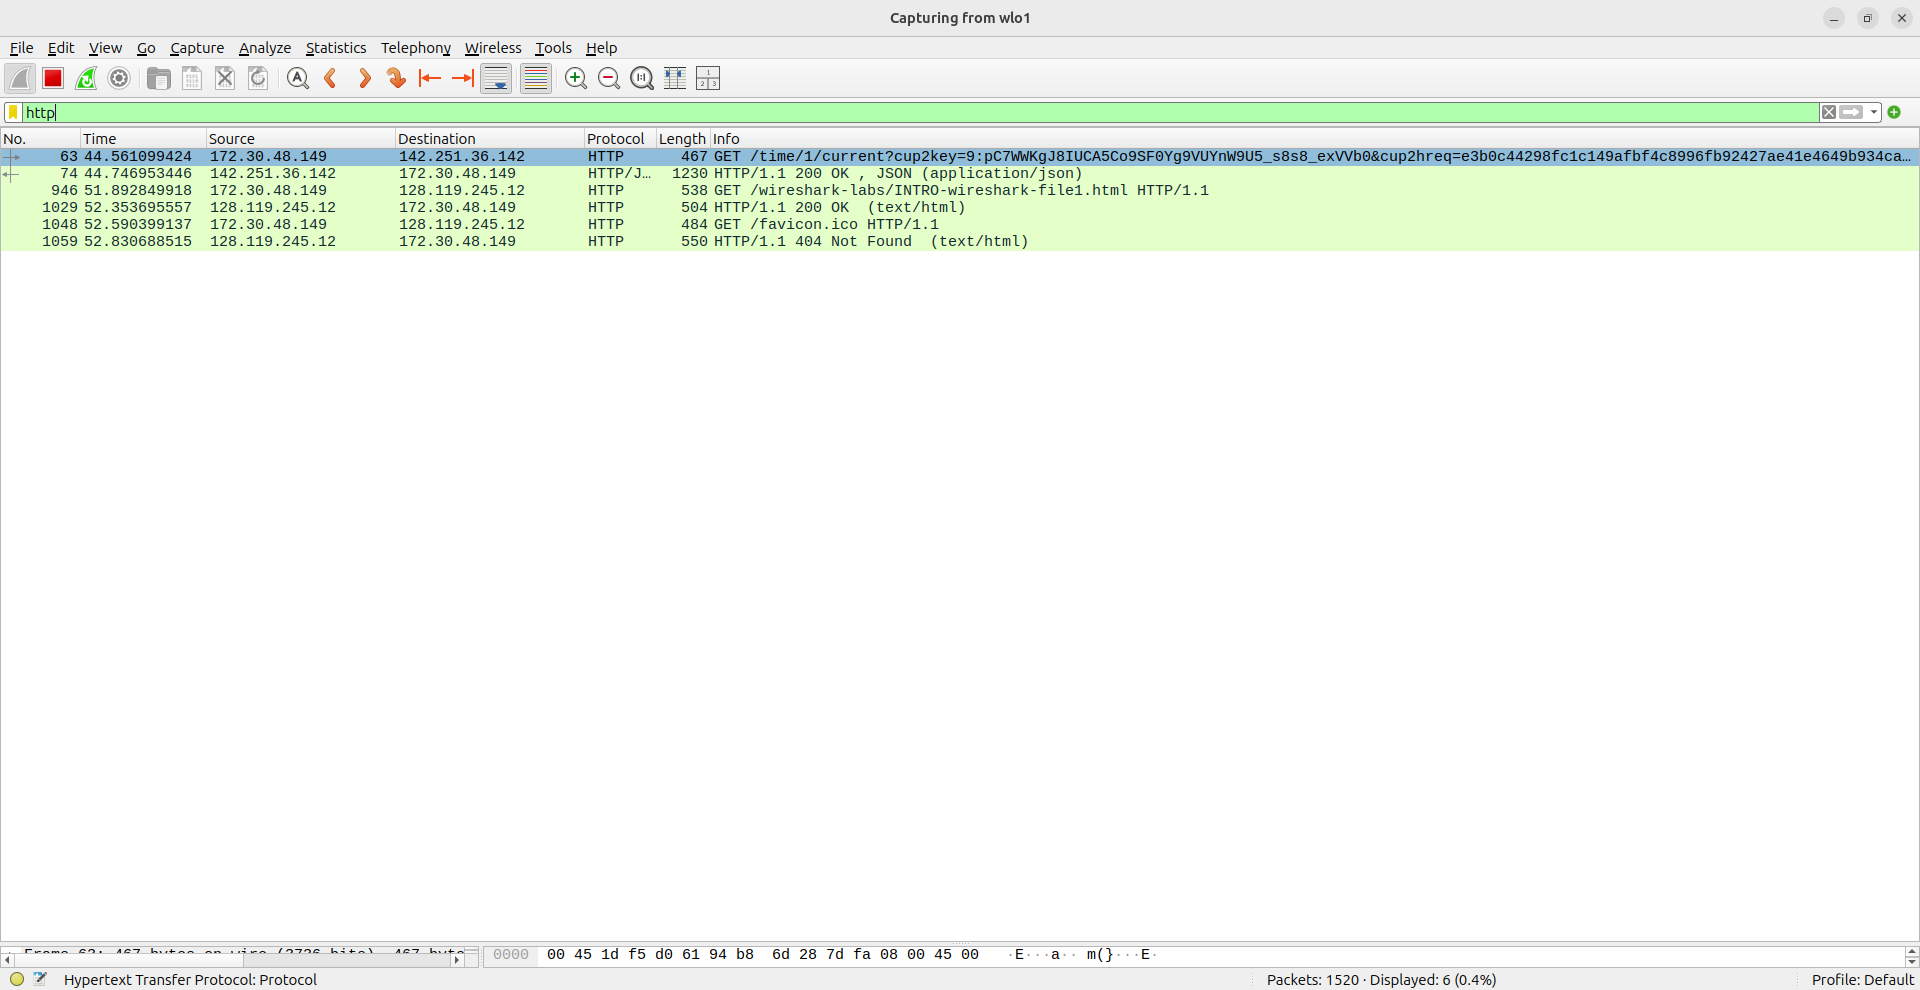
\includegraphics[width=\textwidth]{Template - Student/Content/Pic3.png}
  \caption{\lr{Full request URI} و هدرهاي \lr{HTTP}}
\end{figure}

\begin{figure}[h!]
  \centering
  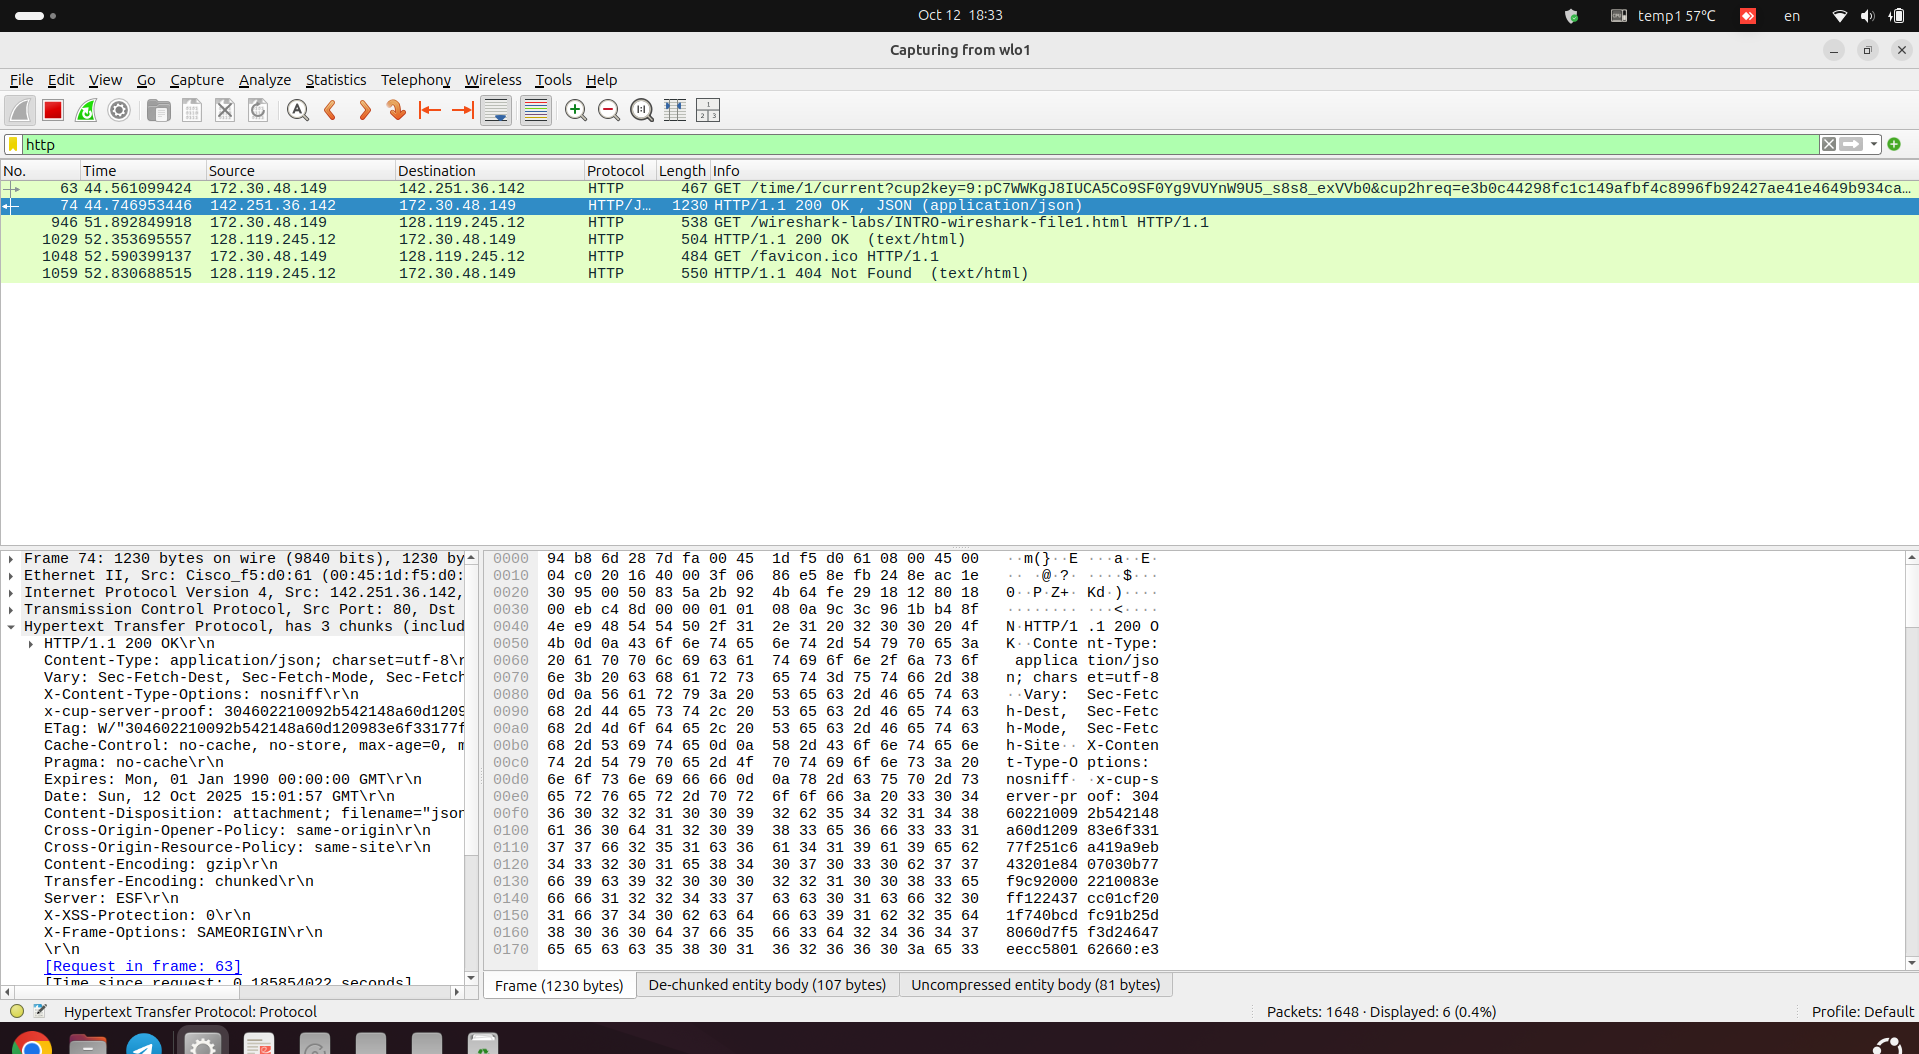
\includegraphics[width=\textwidth]{Template - Student/Content/Pic4.png}
  \caption{پاسخ \lr{HTTP/1.1 200 OK} و \lr{entity body}}
\end{figure}

\begin{figure}[h!]
  \centering
  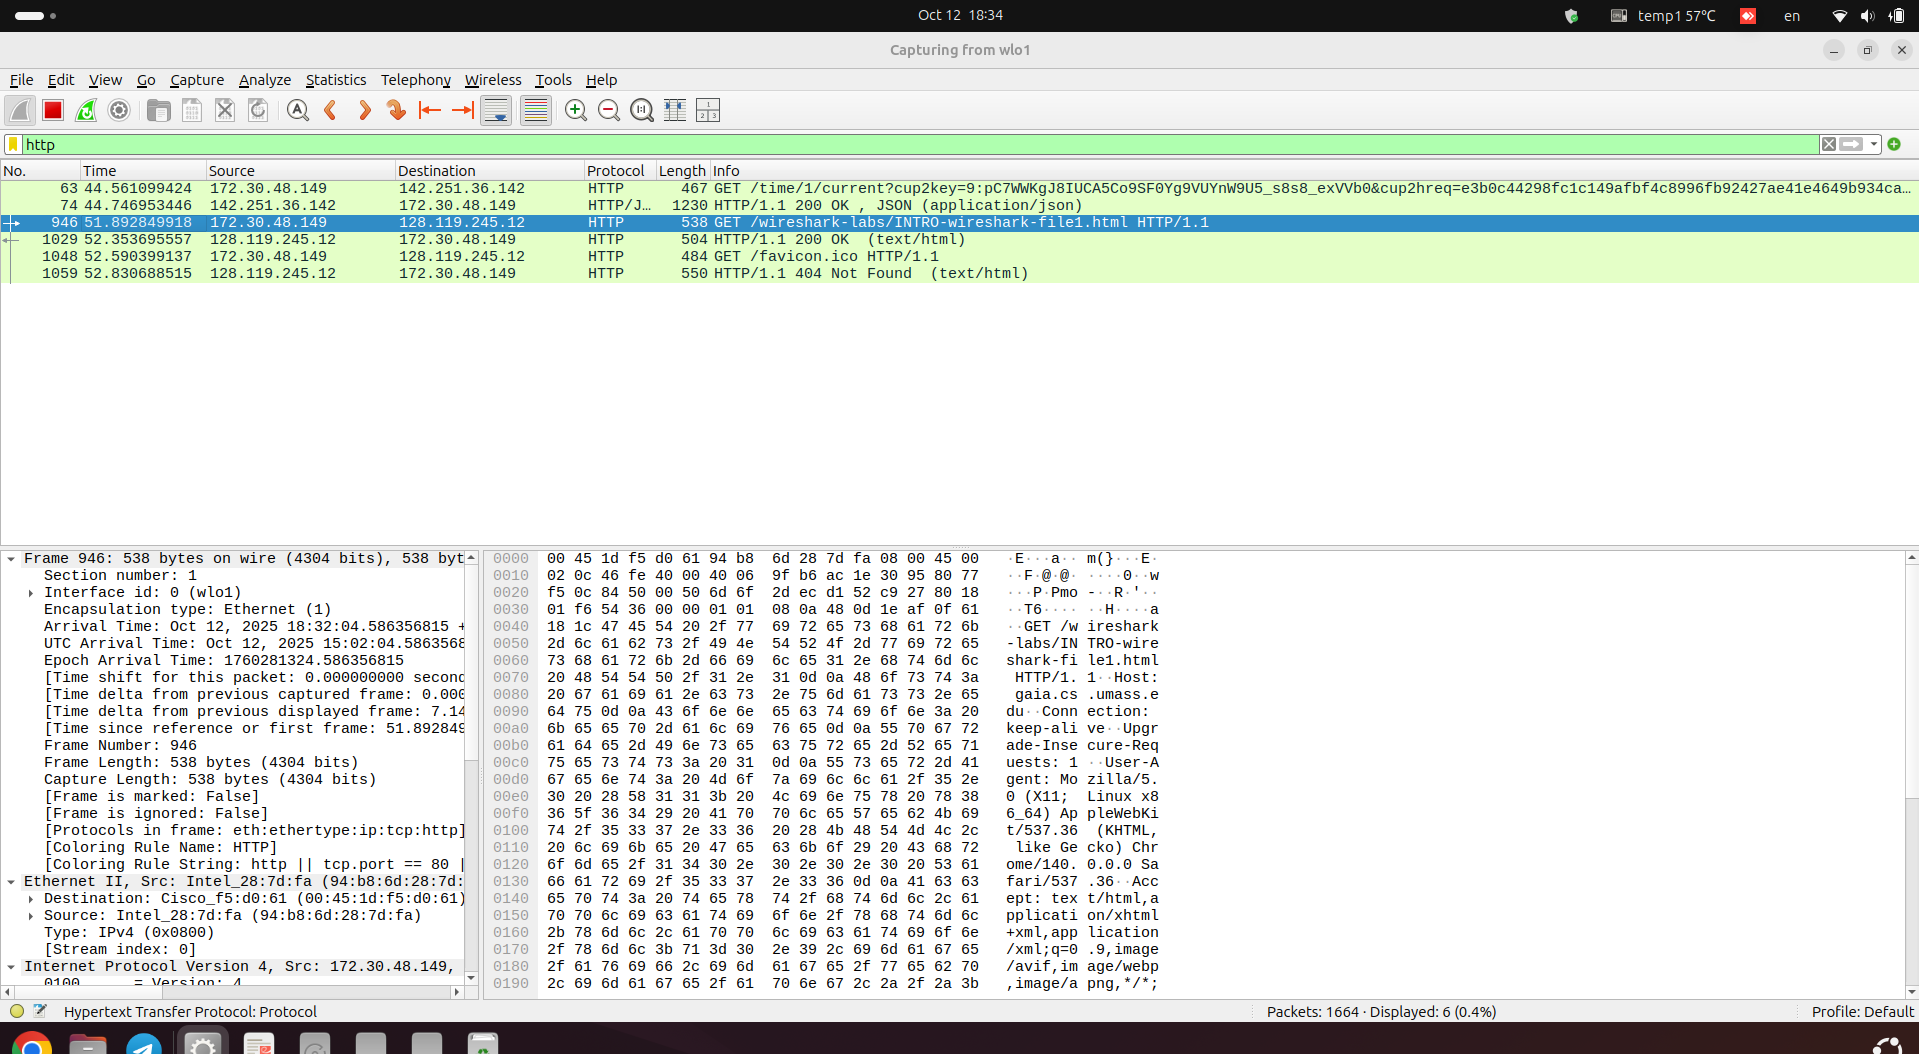
\includegraphics[width=\textwidth]{Template - Student/Content/Pic5.png}
  \caption{جزئيات لايه \lr{TCP} (پورت‌ها، \lr{Seq}/\lr{Ack})}
\end{figure}

\begin{figure}[h!]
  \centering
  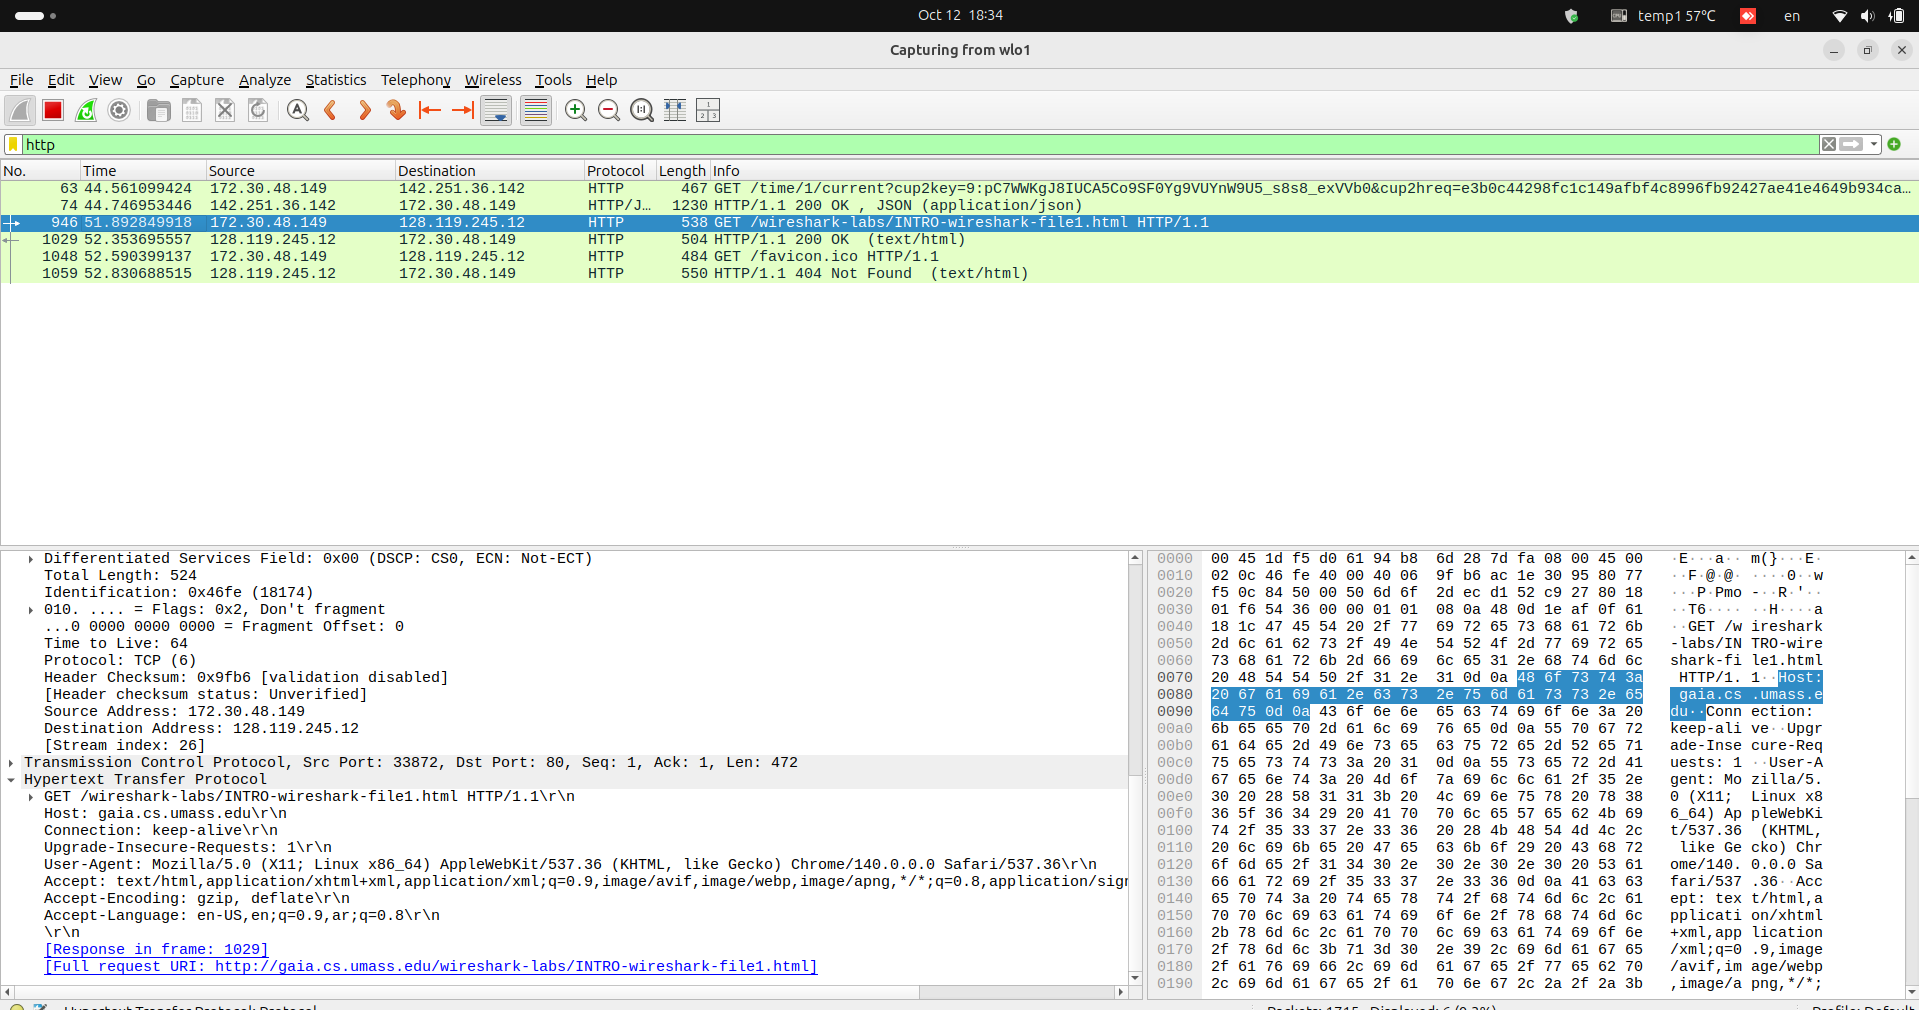
\includegraphics[width=\textwidth]{Template - Student/Content/Pic6.png}
  \caption{\lr{Host: gaia.cs.umass.edu} در هدر \lr{HTTP}}
\end{figure}

\begin{figure}[h!]
  \centering
  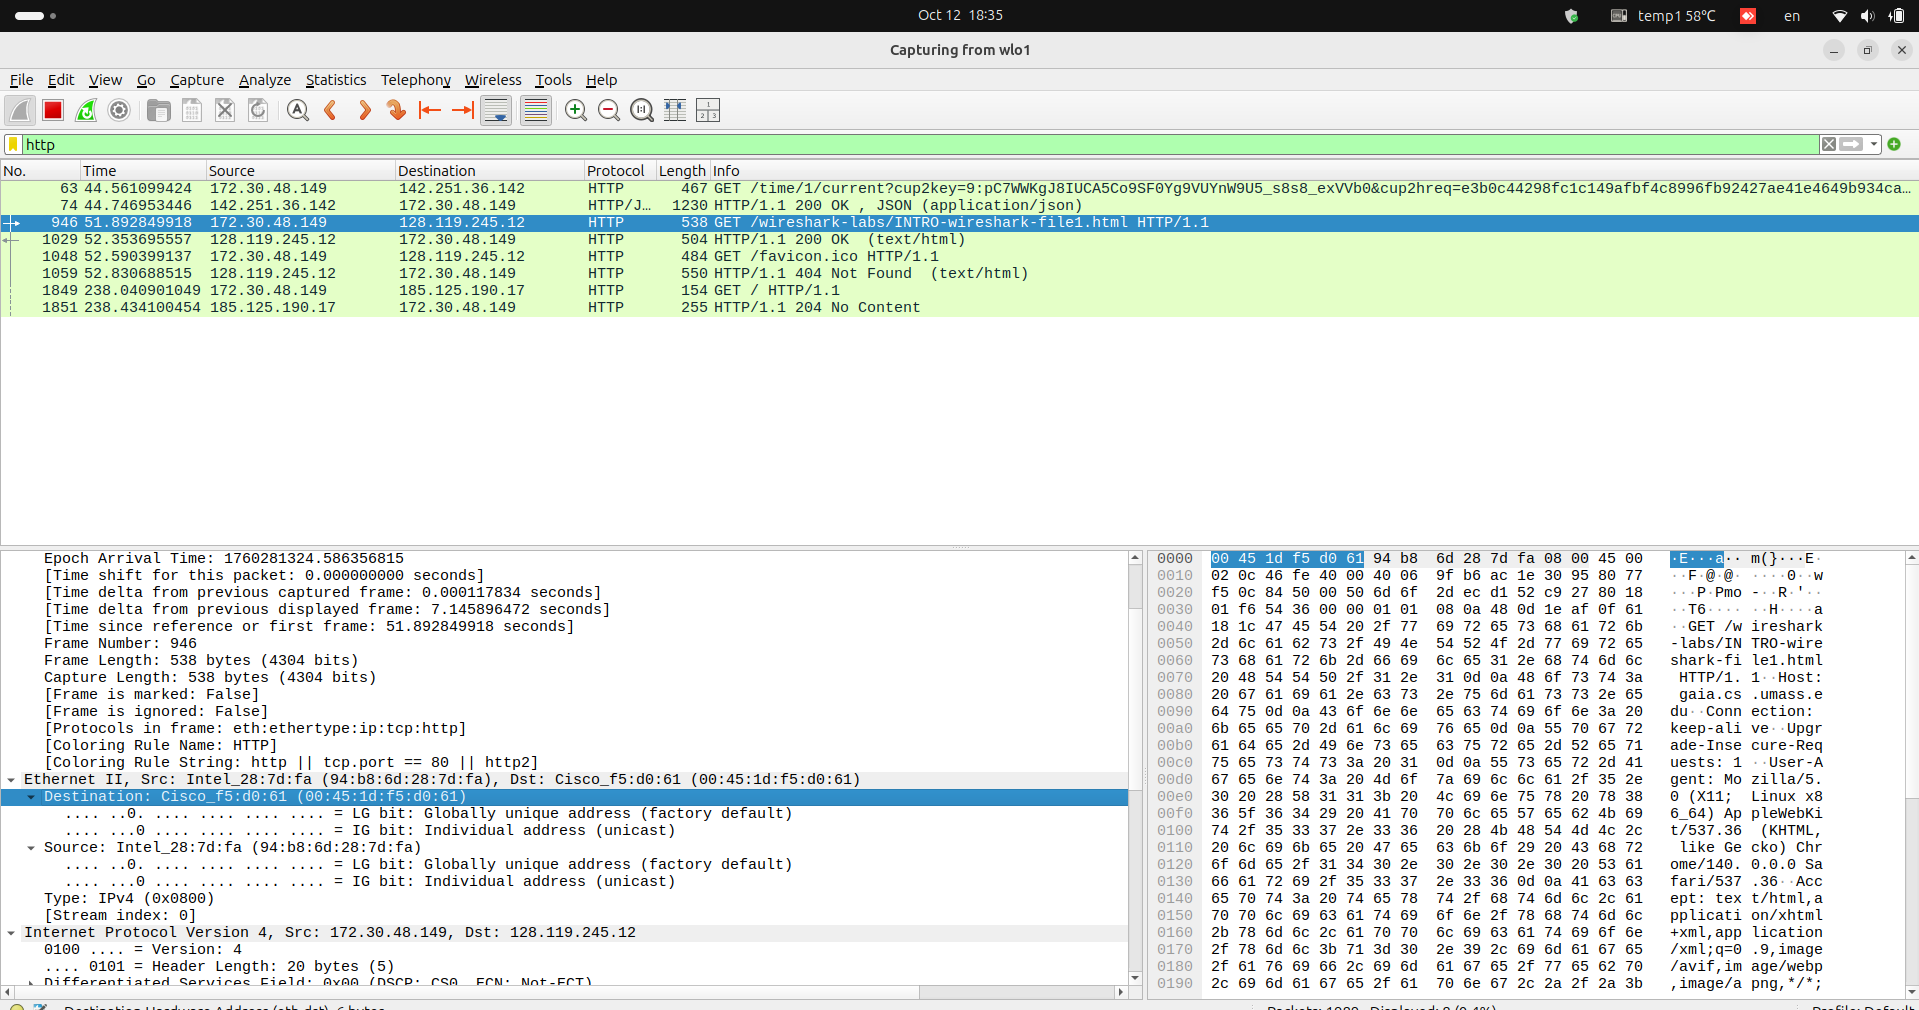
\includegraphics[width=\textwidth]{Template - Student/Content/Pic7.png}
  \caption{تاكيد بر \lr{GET} به \lr{/wireshark-labs/INTRO-wireshark-file1.html}}
\end{figure}

\begin{figure}[h!]
  \centering
  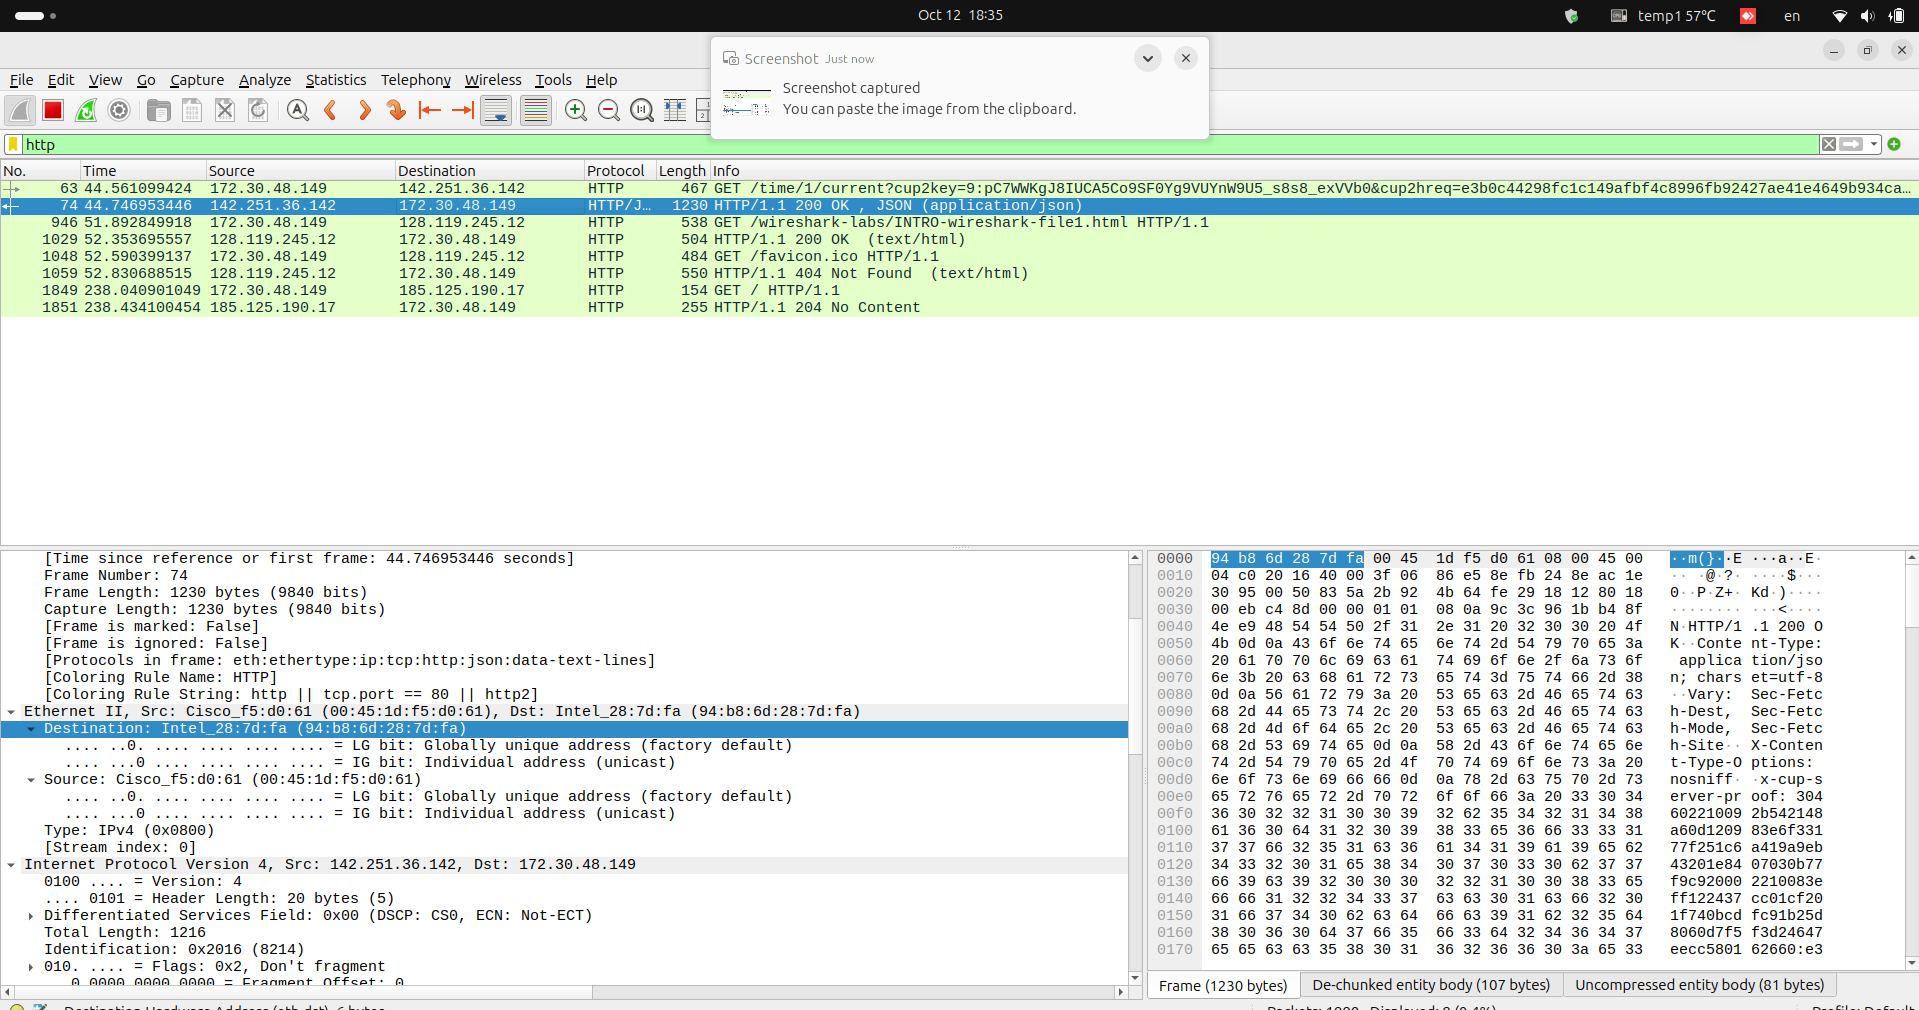
\includegraphics[width=\textwidth]{Template - Student/Content/Pic8.png}
  \caption{نمونه‌هاي ديگر \lr{HTTP}/\lr{JSON} براي مقايسه زمان پاسخ}
\end{figure}